% Provenance (never printed): see sources/outline_sources.md (Year 3:
% dislocation and diffusion creep; flow laws; deformation maps; shear zones and
% kinematic indicators). Brief: sources/book5/BRIEFS.md, ch. 7. Curves from
% figdata/bachelor-3/flow_laws.py. Exercise and problem values in the Book 5
% scratch calculator calc/ch07.py.
\chapter{विरूपण क्रियाविधियाँ और अपरूपण क्षेत्र}\label{ch:b3:deformation-mechanisms}

सतह पर किसी पर्वत का ग्रेनाइट भ्रंशों के साथ टूट जाता है। बीस
किलोमीटर गहराई पर वही ग्रेनाइट कुछ सौ मीटर चौड़े \omterm{def:b3:deformation-mechanisms:shear-zone}{अपरूपण क्षेत्र} में टॉफ़ी की तरह बहता है,
इसके फ़ेल्सपार आँखों जैसे गोल हो जाते हैं, और इसका क्वार्ट्ज़ फीतों की तरह खिंच जाता है।
एक क्रिस्टल बिना टूटे बह सकता है, क्योंकि वह कभी पूर्ण नहीं होता:
वह अपने दोषों के सहारे चलता है, एक बार में परमाणुओं की एक पंक्ति, या परमाणुओं के
एक कण के एक फलक से दूसरे फलक तक विसरण द्वारा। यह अध्याय इन क्रियाविधियों का अनुसरण
क्रिस्टल जालक से लेकर उन नियमों तक करता है जिन्हें भूगतिकी प्रयोग करती है, उन मानचित्रों तक जो बताते हैं कि
कौन-सी क्रियाविधि प्रबल होती है, और उन अपरूपण क्षेत्रों तक जिनमें चट्टान अभिलेखित करती है कि वह कैसे चली।

\begin{recall}
बिंदु दोष, आरेनियस नियम और सक्रियण ऊर्जा रसायन की पुस्तकों के विश्वविद्यालय-स्तर के
खंडों में हैं; विसरण गुणांक भौतिकी की
पुस्तकों में है। प्रतिबल और विकृति, विकृति-दीर्घवृत्त, सरल कर्तन और उसका दीर्घवृत्त
($S_{1,2} = \sqrt{1 + \gamma^2/4} \pm \gamma/2$, अपरूपण दिशा से $\theta'$ पर दीर्घ अक्ष,
जहाँ $\tan2\theta' = 2/\gamma$), गीले क्वार्ट्ज़ाइट और शुष्क ओलिवीन के स्थिरांकों वाला घात-नियम विसर्पण,
सामर्थ्य-आवरण और भंगुर–तन्य संक्रमण पुस्तक 3 (स्नातक वर्ष 1) में, उसके
प्रतिबल, विकृति और प्रवाहिकी पर अध्याय में हैं; पर्णन, रेखन और वर्णनात्मक
मायलोनाइट उसी पुस्तक के भ्रंश, वलन और विन्यास पर अध्याय में हैं।
प्रावार की प्रभावी
श्यानता \cref{ch:b3:mantle-convection} में है।
\end{recall}

\section{क्रिस्टल दोष}

पूर्ण क्रिस्टल को अपरूपित करने के लिए जालक-तल के आर-पार के सभी बंधनों को एक साथ
टूटना होगा, और इसके लिए अपरूपण मापांक के दसवें भाग की कोटि का प्रतिबल चाहिए,
जो प्रावार में लगभग \qty{8e10}{Pa} है
(\cref{ch:b3:mantle-convection} देखिए): हज़ारों मेगापास्कल।
वास्तविक क्रिस्टल कहीं कम प्रतिबल पर विरूपित होने लगते हैं, क्योंकि वे परमाणुओं की एक-एक पंक्ति खिसकाते हैं।

\begin{definition}[अव्यवस्थापन]\label{def:b3:deformation-mechanisms:dislocation}
\emph{अव्यवस्थापन}\index{अव्यवस्थापन (क्रिस्टल दोष)} क्रिस्टल में एक रेखीय दोष है:
क्रिस्टल के भीतर वह सीमा जो जालक-तल के खिसके हुए भाग और न खिसके हुए भाग के बीच होती है।
इसका \emph{बर्गर्स सदिश}
$\mathbf b$ वह खिसकाव है जो यह वहन करता है, किसी जालक-दिशा में एक जालक-अंतराल।
किनारी अव्यवस्थापन में $\mathbf b$ रेखा के लंबवत होता है,
जो परमाणुओं के एक अतिरिक्त अर्ध-तल का किनारा है; पेच अव्यवस्थापन में यह
रेखा के समांतर होता है। अव्यवस्थापन अपने खिसकाव-तल पर \emph{सर्पण} द्वारा चलता है,
और किनारी अव्यवस्थापन \emph{आरोहण} द्वारा उस तल से बाहर निकलता है, जब परमाणु या
रिक्तियाँ उसके अर्ध-तल के किनारे की ओर या वहाँ से विसरित होती हैं।
\end{definition}

\begin{omfigure}
\begin{tikzpicture}[font=\scriptsize, x=0.42cm, y=0.42cm]
% (क) lower half: 10 columns; upper half: 11 columns squeezed over the same width
\foreach \j in {0,...,3} {\foreach \i in {0,...,9} {\fill[gray!70] (\i,\j) circle (0.13);}}
\foreach \j/\s in {4/0.9, 5/0.92, 6/0.94, 7/0.96} {\foreach \i in {0,...,10} {
  \pgfmathsetmacro{\x}{(\i-5)*\s + 4.5}
  \ifnum\i=5 \fill[red!70!black] (\x,\j) circle (0.15); \else \fill[gray!70] (\x,\j) circle (0.13); \fi}}
\draw[thick, blue!60!black] (-0.6,3.5) -- (9.6,3.5);
\node[anchor=east, blue!60!black] at (-0.7,3.5) {खिसकाव-तल};
\draw[red!70!black, very thick] (4.1,3.62) -- (4.9,3.62) (4.5,3.62) -- (4.5,4.2);
\node[red!70!black] at (4.5,8.2) {अतिरिक्त अर्ध-तल};
\draw[->, thick] (1.0,9.2) -- (3.0,9.2) node[right] {$\tau$};
\draw[<-, thick] (6.0,-1.0) -- (8.0,-1.0) node[right] {$\tau$};
% (ख) after glide: the upper half shifted by one spacing
\begin{scope}[shift={(14,0)}]
\foreach \j in {0,...,3} {\foreach \i in {0,...,9} {\fill[gray!70] (\i,\j) circle (0.13);}}
\foreach \j in {4,...,7} {\foreach \i in {1,...,10} {\fill[gray!70] (\i,\j) circle (0.13);}}
\draw[thick, blue!60!black] (-0.6,3.5) -- (10.6,3.5);
\draw[|<->|] (9,8.3) -- (10,8.3) node[midway, above] {$\mathbf b$};
\end{scope}
\node[anchor=north] at (4.5,-1.8) {(क) एक किनारी अव्यवस्थापन};
\node[anchor=north] at (19,-1.8) {(ख) सर्पण के बाद};
\end{tikzpicture}

\par\smallskip{\small (क) एक किनारी \omterm{def:b3:deformation-mechanisms:dislocation}{अव्यवस्थापन}: परमाणुओं का एक अतिरिक्त अर्ध-तल (लाल)
खिसकाव-तल पर समाप्त होता है और अपने किनारे के चारों ओर जालक को विकृत करता है (चिह्न
$\perp$)। अपरूपण प्रतिबल $\tau$ के अंतर्गत यह खिसकाव-तल के साथ एक बार में एक
पंक्ति बंधनों को तोड़कर और फिर से बनाकर सर्पण करता है। (ख) जब यह क्रिस्टल को
पार कर जाता है, तो ऊपरी भाग एक बर्गर्स सदिश $\mathbf b$ जितना खिसक चुका होता है, और
जालक फिर से पूर्ण हो जाता है।}\label{fig:b3:deformation-mechanisms:dislocation}
\end{omfigure}

जालक \omterm{def:b3:deformation-mechanisms:dislocation}{अव्यवस्थापन} के सर्पण का विरोध एक छोटे प्रतिबल से करता है, जिसे
पायर्ल्स प्रतिबल कहते हैं और जो बंधनों की सामर्थ्य और दिशा पर निर्भर करता है:
इसी कारण किसी खनिज के कुछ खिसकाव तंत्र सरल और कुछ कठिन होते हैं। जैसे-जैसे
क्रिस्टल विरूपित होता है, \omterm{def:b3:deformation-mechanisms:dislocation}{अव्यवस्थापन} बढ़ते हैं और उलझते हैं; वे एक-दूसरे को रोकते हैं, और
क्रिस्टल कठोर हो जाता है, जब तक वे बाधाओं के चारों ओर आरोहण न कर सकें या परस्पर विलुप्त न हो जाएँ, जिसके लिए
विसरण चाहिए, और इसलिए ऊष्मा।

\section{विसर्पण की क्रियाविधियाँ}

\begin{definition}[विसर्पण की क्रियाविधियाँ]\label{def:b3:deformation-mechanisms:creep}
\emph{अव्यवस्थापन विसर्पण}\index{अव्यवस्थापन विसर्पण} में क्रिस्टल अव्यवस्थापनों के
सर्पण से विरूपित होते हैं, और आरोहण उन्हें बाधाओं से मुक्त करता है।
\emph{विसरण विसर्पण}\index{विसरण विसर्पण} में वे परमाणुओं के विसरण से आकार बदलते हैं,
जालक के आर-पार (नैबैरो--हेरिंग विसर्पण) या कण-सीमाओं के साथ (कोबल विसर्पण),
अधिकतम अभिलंब प्रतिबल वाले फलकों से
न्यूनतम वाले फलकों की ओर। \emph{कण-सीमा सर्पण}\index{कण-सीमा सर्पण} में
कण अपनी सीमाओं के साथ एक-दूसरे के पास से सरकते हैं, और बने अंतराल
विसरण या \omterm{def:b3:deformation-mechanisms:dislocation}{अव्यवस्थापन} विसर्पण से भरे जाते हैं।
\emph{दाब विलयन}\index{दाब विलयन} में पदार्थ उच्च प्रतिबल वाले फलकों पर एक
तरल फिल्म में घुलता है और जहाँ प्रतिबल कम है वहाँ जमा होता है, या
दूर ले जाया जाता है।
\end{definition}

\begin{proposition}[विसरण विसर्पण की कण-आकार निर्भरता]\label{prop:b3:deformation-mechanisms:grain-size}
कम प्रतिबल $\sigma$ पर, कण-आकार $d$ वाली चट्टान इस दर से विसरण द्वारा विसर्पित होती है
\[
  \dot\varepsilon \approx B_L\frac{D_L\Omega}{k_BT}\frac{\sigma}{d^2}
  \quad\text{(जालक के आर-पार)},\qquad
  \dot\varepsilon \approx B_B\frac{\delta D_B\Omega}{k_BT}\frac{\sigma}{d^3}
  \quad\text{(सीमाओं के साथ)},
\]
जहाँ $D_L$ और $D_B$ क्रमशः जालक और सीमाओं में विसरण गुणांक हैं,
$\delta$ सीमा की चौड़ाई है, $\Omega$ एक परमाणु का आयतन है,
$k_B$ बोल्ट्ज़मान स्थिरांक है और $B_L$, $B_B$ ऐसी संख्याएँ हैं जिनकी कोटि दस है और जो
कणों के आकार पर निर्भर करती हैं।
\end{proposition}

\begin{proof}
किसी फलक पर अभिलंब प्रतिबल $\sigma$ वहाँ एक रिक्ति बनाने के लिए आवश्यक कार्य को
$\sigma\Omega$ से बदल देता है, इसलिए रिक्तियों का सांद्रण $C$ तनाव और संपीड़न में स्थित फलकों के बीच
भिन्न होता है, और यह अंतर $\Delta C \approx C\sigma\Omega/
(k_BT)$ होता है, जब $\sigma\Omega \ll k_BT$ हो। कोटि $d$ की दूरी पर
रिक्तियों का विसरण-प्रवाह, और इसलिए परमाणुओं का उल्टी दिशा में प्रवाह, प्रति इकाई क्षेत्रफल कोटि $D\Delta
C/d$ का होता है। जालक के आर-पार यह प्रवाह कोटि
$d^2$ के क्षेत्रफल से होकर गुज़रता है, और सीमाओं के साथ कोटि $\delta d$ के क्षेत्रफल से। प्रति इकाई समय में स्थानांतरित आयतन
कण के आयतन $d^3$ से भाग देने पर वह विकृति-दर होती है, जिसकी कोटि
$(D_L\sigma\Omega/k_BT)\,d^2/(d\cdot d^3) = D_L\sigma\Omega/(k_BTd^2)$ जालक में, और
$(D_B\sigma\Omega/k_BT)\,\delta d/(d\cdot d^3) = \delta D_B
\sigma\Omega/(k_BTd^3)$ सीमाओं में है। गुणनफल $C\,D$ वह
स्व-विसरण गुणांक है जिसे कथन में $D$ लिखा गया है।
\end{proof}

\omterm{def:b3:deformation-mechanisms:creep}{विसरण विसर्पण} प्रतिबल में रैखिक होता है, वह एक वास्तविक श्यान प्रवाह है, और वह सूक्ष्म-कणिका
चट्टान में तेज़ होता है: कण-आकार आधा करने पर कोबल विसर्पण आठ गुना तेज़ हो जाता है
(नीचे का चित्र)। \omterm{def:b3:deformation-mechanisms:creep}{अव्यवस्थापन विसर्पण} कण-आकार पर निर्भर नहीं करता, परंतु
प्रतिबल की उच्च घात के साथ बढ़ता है।

\begin{omfigure}
\begin{tikzpicture}[font=\scriptsize, x=1cm, y=1cm]
\foreach \cx/\lab in {0/{(क) जालक से होकर}, 6/{(ख) सीमाओं के साथ}} {
  \begin{scope}[shift={(\cx,0)}]
  \draw[thick, fill=gray!10] (-1.6,-1.1) -- (-0.6,-1.7) -- (1.0,-1.6) -- (1.7,-0.4) -- (1.5,1.0) -- (0.4,1.7) -- (-1.2,1.3) -- (-1.8,0.2) -- cycle;
  \draw[->, very thick, red!70!black] (0,2.6) -- (0,1.9);
  \draw[->, very thick, red!70!black] (0,-2.6) -- (0,-1.9);
  \node[red!70!black] at (0.45,2.45) {$\sigma$};
  \draw[<-, very thick, gray] (2.7,0.3) -- (2.0,0.3);
  \draw[<-, very thick, gray] (-2.8,-0.3) -- (-2.1,-0.3);
  \node[anchor=north] at (0,-2.8) {\lab};
  \end{scope}
}
\foreach \sx in {1,-1} {\foreach \y in {-0.5,0.5} {
  \draw[->, blue!60!black, thick] (0.15*\sx,1.25) .. controls (0.5*\sx,\y+0.6) and (0.9*\sx,\y+0.15) .. (1.45*\sx,\y);
  \draw[->, blue!60!black, thick] (0.15*\sx,-1.25) .. controls (0.5*\sx,\y-0.6) and (0.9*\sx,\y-0.15) .. (1.45*\sx,\y);
}}
\draw[->, blue!60!black, thick] (6.4,1.62) -- (7.45,1.05) -- (7.65,0.2);
\draw[->, blue!60!black, thick] (5.9,1.45) -- (4.85,1.35) -- (4.25,0.3);
\draw[->, blue!60!black, thick] (6.9,-1.62) -- (7.0,-1.6) -- (7.6,-0.6);
\draw[->, blue!60!black, thick] (5.6,-1.6) -- (5.4,-1.68) -- (4.45,-1.15) -- (4.25,-0.3);
\end{tikzpicture}

\par\smallskip{\small $\sigma$ के अनुदिश छोटे हुए कण का \omterm{def:b3:deformation-mechanisms:creep}{विसरण विसर्पण}। परमाणु
सबसे अधिक संपीड़न वाले फलकों से हटते हैं और सबसे कम संपीड़न वाले फलकों पर
जुड़ते हैं (नीले तीर), जिससे कण चपटा होकर लंबा हो जाता है (धूसर तीर): (क)
कण के आंतरिक भाग से, नैबैरो--हेरिंग विसर्पण; (ख) उसकी सीमाओं के साथ,
कोबल विसर्पण।}\label{fig:b3:deformation-mechanisms:diffusion}
\end{omfigure}

विरूपित क्रिस्टल विरूपण के दौरान स्वयं को भी ठीक कर लेते हैं।

\begin{definition}[पुनर्प्राप्ति, उपकण, गतिक पुनःक्रिस्टलन]\label{def:b3:deformation-mechanisms:recrystallisation}
\emph{पुनर्प्राप्ति}\index{पुनर्प्राप्ति (क्रिस्टल प्लास्टिसिटी)} वह पुनर्विन्यास है, जो
अव्यवस्थापनों का आरोहण और क्रॉस-स्लिप द्वारा निम्न-ऊर्जा संरचनाओं में होता है, और उनका
विलोपन। दीवारों में व्यवस्थित \omterm{def:b3:deformation-mechanisms:dislocation}{अव्यवस्थापन} एक कण को
\emph{उपकणों}\index{उपकण}, कण के वे भाग हैं जिनकी जालकें
एक-दूसरे से कुछ अंश तक झुकी होती हैं। \emph{गतिक
पुनःक्रिस्टलन}\index{गतिक पुनःक्रिस्टलन} विरूपण के दौरान विकृत कणों को
उन नए कणों से बदलने की प्रक्रिया है जिनमें कम \omterm{def:b3:deformation-mechanisms:dislocation}{अव्यवस्थापन} होते हैं, या तो
उपकणों के घूमने से, जब तक वे कण न बन जाएँ, या
कण-सीमाओं के अधिक विकृत पड़ोसियों में प्रवास से।
\end{definition}

\begin{definition}[क्रिस्टलीय अधिमान्य अभिविन्यास]\label{def:b3:deformation-mechanisms:cpo}
किसी चट्टान में \emph{क्रिस्टलीय अधिमान्य अभिविन्यास}\index{क्रिस्टलीय अधिमान्य अभिविन्यास}
(CPO) तब होता है, जब उसके कणों की जालकें यादृच्छिक नहीं होतीं,
बल्कि विरूपण द्वारा तय दिशाओं के आसपास समूहित होती हैं; \omterm{def:b3:deformation-mechanisms:creep}{अव्यवस्थापन
विसर्पण} इसे उत्पन्न करता है, प्रत्येक कण की सर्पण-प्रणालियों को प्रवाह की ओर घुमाकर।
\end{definition}

CPO वाली चट्टान अपने क्रिस्टलों की अनिसॉट्रॉपी ग्रहण करती है: उसकी भूकंपीय गति,
उदाहरण के लिए, दिशा पर निर्भर करती है, और इसी से भूकंपविज्ञान गहरे प्रावार का विन्यास
देख पाता है। \omterm{def:b3:deformation-mechanisms:creep}{विसरण विसर्पण} और \omterm{def:b3:deformation-mechanisms:creep}{कण-सीमा सर्पण}, जो कणों को स्वतंत्र रूप से
घूमने देते हैं, इसे नहीं बनाते।

\section{प्रवाह नियम}

\begin{definition}[प्रवाह नियम, प्रतिबल घातांक, समजात तापमान]\label{def:b3:deformation-mechanisms:flow-law}
\emph{प्रवाह नियम}\index{प्रवाह नियम} किसी एक क्रियाविधि से विरूपित हो रही चट्टान की विकृति-दर को
अवकल प्रतिबल $\sigma$, कण-आकार
$d$, तापमान $T$ और दाब $P$ के फलन के रूप में देता है:
\[
  \dot\varepsilon = A\,\sigma^nd^{-m}\exp\Bigl(-\frac{E + PV}{RT}\Bigr),
\]
जहाँ $A$, $n$, $m$, सक्रियण ऊर्जा $E$ और सक्रियण आयतन $V$
प्रयोगशाला में मापे जाते हैं। \emph{प्रतिबल घातांक}\index{प्रतिबल घातांक}
$n$ है, कण-आकार घातांक $m$। किसी खनिज का \emph{समजात
तापमान}\index{समजात तापमान} $T/T_m$ है, उसका
निरपेक्ष तापमान, उसके निरपेक्ष गलन तापमान से भाग देकर प्राप्त होता है।
\end{definition}

यहाँ प्रयुक्त नियमों में \omterm{def:b3:deformation-mechanisms:creep}{अव्यवस्थापन विसर्पण} के लिए $n$ का मान 3.5 या 4 होता है और $m = 0$;
\omterm{def:b3:deformation-mechanisms:creep}{विसरण विसर्पण} में $n = 1$ और $m = 2$ या 3 होता है (\cref{prop:b3:deformation-mechanisms:grain-size} देखिए)।
\omterm{def:b3:deformation-mechanisms:flow-law}{समजात तापमान} 1 के निकट पहुँचने पर विसर्पण बढ़ता है। फ़ॉर्स्टेराइट \qty{1890}{\celsius} पर गलता है, इसलिए \qty{1300}{\celsius} पर प्रावार
$T/T_m = 0.73$ पर होता है; \qty{-10}{\celsius} पर बर्फ़ 0.96 पर होती है, इसीलिए
हिमनद बहते हैं। यहाँ प्रयुक्त ओलिवीन के मान एक व्यापक रूप से उपयोग में आने वाले
प्रयोगशाला संकलन के हैं: \omterm{def:b3:deformation-mechanisms:creep}{अव्यवस्थापन विसर्पण} में शुष्क ओलिवीन के लिए, $A =
\num{1.1e5}$, $n = 3.5$, $E = \qty{530}{kJ.mol^{-1}}$, $V =
\qty{14}{cm^3.mol^{-1}}$; \omterm{def:b3:deformation-mechanisms:creep}{विसरण विसर्पण} में, $A = 10^{9.2}$, $n = 1$, $m = 3$,
$E = \qty{375}{kJ.mol^{-1}}$, $V = \qty{5}{cm^3.mol^{-1}}$ (प्रतिबल मेगापास्कल में,
कण-आकार माइक्रोमीटर में, समय सेकंड में); आर्द्र क्वार्ट्ज़ाइट के मान
पुस्तक 3 (स्नातक वर्ष 1) में हैं। जल ओलिवीन को दुर्बल करता है: लगभग
\qty{300}{MPa} की जल-फ़ुगैसिटी पर ओलिवीन समुच्चय शुष्क समुच्चयों की तुलना में
\omterm{def:b3:deformation-mechanisms:creep}{अव्यवस्थापन विसर्पण} में पाँच से छह गुना तेज़ विसर्पित होते हैं, और \omterm{def:b3:deformation-mechanisms:creep}{विसरण विसर्पण} में पाँच गुना तेज़।
% ledger: bowen14:mgo-sio2, azuma17:olivine, lopez:flow-laws, codata:R, mk00:diffusion, mk00:dislocation

\begin{proposition}[प्रभावी श्यानता]\label{prop:b3:deformation-mechanisms:viscosity}
\omterm{def:b3:deformation-mechanisms:flow-law}{प्रवाह नियम} $\dot\varepsilon = A'\sigma^n$ का पालन करने वाली चट्टान, दिए गए $T$, $P$ और
$d$ पर उसकी प्रभावी श्यानता होती है
\[
  \eta_{\mathrm{eff}} = \frac{\sigma}{2\dot\varepsilon}
  = \tfrac12A'^{-1/n}\,\dot\varepsilon^{(1-n)/n}:
\]
$n > 1$ के लिए यह तब घटती है जब चट्टान तेज़ी से विरूपित होती है।
\end{proposition}

\begin{proof}
न्यूटनीय तरल के लिए, श्यानता की परिभाषा से, एकाक्षीय प्रवाह में $\sigma = 2\eta\dot\varepsilon$
$\eta_{\mathrm{eff}}$ उस न्यूटनीय तरल की श्यानता है जो समान प्रतिबल के
अंतर्गत उसी दर से बहता।
$\sigma = (\dot\varepsilon/A')^{1/n}$ रखने पर दूसरा रूप प्राप्त होता है।
\end{proof}

\qty{400}{\celsius} पर गीला क्वार्ट्ज़ाइट, \qty{e-14}{s^{-1}} की दर से बहने के लिए
\qty{65}{MPa} प्रतिबल चाहिए और इसकी प्रभावी श्यानता \qty{3.3e21}{Pa.s} होती है;
\qty{500}{\celsius} पर \qty{18}{MPa} और \qty{9e20}{Pa.s}: सौ अंश का तापमान अंतर
प्रतिबल को तीन गुने से अधिक घटा देता है (नीचे का चित्र)। शुष्क ओलिवीन
\qty{1100}{\celsius} और \qty{1}{GPa} पर केवल \qty{3}{MPa} प्रतिबल चाहिए।
पुस्तक 3 (स्नातक वर्ष 1) के सामर्थ्य-आवरण ठीक इन्हीं नियमों से बनते हैं।

\begin{omfigure}
\begin{tikzpicture}
\begin{groupplot}[group style={group size=2 by 1, horizontal sep=1.6cm},
  omrecord, width=0.47\linewidth, height=0.47\linewidth, xmode=log,
  xmin=1, xmax=1000, ymin=-20, ymax=-6, xlabel={अवकल प्रतिबल (MPa)},
  legend style={font=\scriptsize, at={(0.97,0.03)}, anchor=south east, legend columns=1}]
\nextgroupplot[ylabel={$\log_{10}\dot\varepsilon$ (\unit{s^{-1}})}, title={(क) गीला क्वार्ट्ज़ाइट},
  title style={font=\small}]
% computed in figdata/bachelor-3/flow_laws.py; ledger: lopez:flow-laws, azuma17:olivine
\addplot[omDef, thick] table[x=s, y=r600] {figdata/out/bachelor-3-flow_laws-quartz.dat};
\addlegendentry{\qty{600}{\celsius}}
\addplot[red!70!black, thick, densely dashed] table[x=s, y=r500] {figdata/out/bachelor-3-flow_laws-quartz.dat};
\addlegendentry{\qty{500}{\celsius}}
\addplot[black, thick, densely dotted] table[x=s, y=r400] {figdata/out/bachelor-3-flow_laws-quartz.dat};
\addlegendentry{\qty{400}{\celsius}}
\draw[gray] (axis cs:1,-14) -- (axis cs:1000,-14);
\nextgroupplot[title={(ख) शुष्क ओलिवीन, \qty{1}{GPa}}, title style={font=\small}]
\addplot[omDef, thick] table[x=s, y=r1300] {figdata/out/bachelor-3-flow_laws-olivine.dat};
\addlegendentry{\qty{1300}{\celsius}}
\addplot[red!70!black, thick, densely dashed] table[x=s, y=r1100] {figdata/out/bachelor-3-flow_laws-olivine.dat};
\addlegendentry{\qty{1100}{\celsius}}
\addplot[black, thick, densely dotted] table[x=s, y=r900] {figdata/out/bachelor-3-flow_laws-olivine.dat};
\addlegendentry{\qty{900}{\celsius}}
\draw[gray] (axis cs:1,-14) -- (axis cs:1000,-14);
\end{groupplot}
\end{tikzpicture}

\par\smallskip{\small \omterm{def:b3:deformation-mechanisms:creep}{अव्यवस्थापन विसर्पण} के \omterm{def:b3:deformation-mechanisms:flow-law}{प्रवाह नियम}: विकृति-दर बनाम प्रतिबल, तीन
तापमानों पर। इन अक्षों पर ढलान \omterm{def:b3:deformation-mechanisms:flow-law}{प्रतिबल घातांक} है, क्वार्ट्ज़ाइट के लिए 4 और
ओलिवीन के लिए 3.5; धूसर रेखा एक भूवैज्ञानिक विकृति-दर दर्शाती है,
\qty{e-14}{s^{-1}}। ओलिवीन को लगभग \qty{600}{\celsius} अधिक तापमान चाहिए
क्वार्ट्ज़ की तरह उतनी ही आसानी से बहने के लिए।}\label{fig:b3:deformation-mechanisms:flow-laws}
\end{omfigure}

\section{विरूपण-क्रियाविधि मानचित्र}

कई क्रियाविधियाँ समानांतर चलती हैं, और सबसे तेज़ क्रियाविधि ही विरूपण को संचालित करती है।

\begin{definition}[विरूपण-क्रियाविधि मानचित्र]\label{def:b3:deformation-mechanisms:deformation-map}
किसी खनिज या चट्टान का \emph{विरूपण-क्रियाविधि मानचित्र}\index{विरूपण-क्रियाविधि मानचित्र}
ऐसा आरेख है जिसके अक्षों पर प्रतिबल, कण-आकार और तापमान में से दो चर लिए जाते हैं,
और वे क्षेत्र दिखाता है जिनमें प्रत्येक क्रियाविधि सबसे तेज़ होती है,
तथा कुल विकृति-दर के समोच्च भी।
\end{definition}

\begin{proposition}[क्रियाविधि-सीमा]\label{prop:b3:deformation-mechanisms:boundary}
दिए गए $T$ और $P$ पर, \omterm{def:b3:deformation-mechanisms:creep}{अव्यवस्थापन विसर्पण} ($A_1$, $n_1$, $E_1$, $V_1$, कोई
कण-आकार पर निर्भरता नहीं) और \omterm{def:b3:deformation-mechanisms:creep}{विसरण विसर्पण} ($A_2$, $n_2 = 1$, $m$, $E_2$, $V_2$)
इस प्रतिबल पर समान तेज़ी से चलते हैं:
\[
  \sigma_b = \biggl(\frac{A_2d^{-m}}{A_1}
  \exp\frac{(E_1 - E_2) + P(V_1 - V_2)}{RT}\biggr)^{1/(n_1 - 1)} ,
\]
अतः सीमा कण-आकार और प्रतिबल के लघुगणकीय अक्षों पर ढलान $-m/(n_1 - 1)$ वाली सीधी रेखा होती है;
इसके ऊपर \omterm{def:b3:deformation-mechanisms:creep}{अव्यवस्थापन विसर्पण} प्रबल होता है।
\end{proposition}

\begin{proof}
दोनों प्रवाह नियमों को बराबर रखकर $\sigma$ के लिए हल किया जाता है। $\sigma_b$ से ऊपर
दोनों दरों का अनुपात, जो $\sigma^{n_1 - 1}$ के समानुपाती है, 1 से अधिक हो जाता है।
\end{proof}

\qty{1100}{\celsius} और \qty{2}{GPa} पर शुष्क ओलिवीन की सीमा
\qty{1}{mm} कण-आकार के लिए \qty{5}{MPa} पर, और
\qty{100}{\micro m} के लिए \qty{79}{MPa} पर स्थित है (नीचे का चित्र)। सूक्ष्म-कण प्रावार विसरण से विसर्पित होता है,
स्थूल-कण प्रावार \omterm{def:b3:deformation-mechanisms:dislocation}{अव्यवस्थापन} से विसर्पित होता है; प्रयोगशाला और भूभौतिकीय साक्ष्य
संकेत देते हैं कि ऊपरी प्रावार में दोनों व्यवस्थाएँ होती हैं: गर्म, उथला प्रावार
\omterm{def:b3:deformation-mechanisms:creep}{अव्यवस्थापन विसर्पण} से विसर्पित होता है, और ठंडा या गहरा \omterm{def:b3:deformation-mechanisms:creep}{विसरण विसर्पण} से, और यह कि जहाँ
प्रतिबल बढ़ता है और कण सिकुड़ते हैं, वहाँ सीमा के निकट का प्रावार दुर्बल हो जाता है
और विरूपण स्थानीकृत हो जाता है।
% ledger: azuma17:olivine, karato93:transitions

\begin{omfigure}
\begin{tikzpicture}
\begin{axis}[omrecord, xmode=log, ymode=log, width=0.78\linewidth, height=0.58\linewidth,
  xmin=10, xmax=1e4, ymin=0.01, ymax=1000, xlabel={कण-आकार (\unit{\micro m})},
  ylabel={अवकल प्रतिबल (MPa)}, clip=true]
% computed in figdata/bachelor-3/flow_laws.py; ledger: azuma17:olivine
\addplot[black, very thick] table[x=d, y=s] {figdata/out/bachelor-3-flow_laws-mapbound.dat};
\foreach \c in {16,14,12,10} {
  \addplot[omDef, thick] table[x=d, y=s\c] {figdata/out/bachelor-3-flow_laws-mapcont.dat};
}
\node[font=\scriptsize, fill=white, inner sep=1pt] at (axis cs:7000,1.15) {$10^{-16}$};
\node[font=\scriptsize, fill=white, inner sep=1pt] at (axis cs:7000,4.2) {$10^{-14}$};
\node[font=\scriptsize, fill=white, inner sep=1pt] at (axis cs:7000,15.7) {$10^{-12}$};
\node[font=\scriptsize, fill=white, inner sep=1pt] at (axis cs:4200,58) {$10^{-10}\,\unit{s^{-1}}$};
\node[font=\small, anchor=north east] at (axis cs:9000,600) {अव्यवस्थापन विसर्पण};
\node[font=\small, anchor=south west] at (axis cs:1500,0.013) {विसरण विसर्पण};
\end{axis}
\end{tikzpicture}

\par\smallskip{\small शुष्क ओलिवीन का \omterm{def:b3:deformation-mechanisms:deformation-map}{विरूपण-क्रियाविधि मानचित्र},
\qty{1100}{\celsius} और \qty{2}{GPa} पर। मोटी रेखा उन क्षेत्रों को अलग करती है जहाँ
\omterm{def:b3:deformation-mechanisms:creep}{अव्यवस्थापन विसर्पण} (ऊपर) या \omterm{def:b3:deformation-mechanisms:creep}{विसरण विसर्पण} (नीचे) अधिक तेज़ होता है; पतली रेखाएँ
कुल विकृति-दर के समोच्च हैं; समतल भाग वहाँ हैं जहाँ \omterm{def:b3:deformation-mechanisms:creep}{अव्यवस्थापन विसर्पण}, जो
कण-आकार की परवाह नहीं करता, प्रधान होता है।}\label{fig:b3:deformation-mechanisms:map}
\end{omfigure}

\omterm{def:b3:deformation-mechanisms:recrystallisation}{गतिक पुनःक्रिस्टलन} से बना कण-आकार प्रतिबल पर निर्भर करता है,
और यही बात कणों को एक प्रतिबल-मापी बना देती है।

\begin{definition}[पुरा-दाबमापी]\label{def:b3:deformation-mechanisms:piezometer}
\emph{पुरा-दाबमापी}\index{पुरा-दाबमापी} एक विरूपित चट्टान की ऐसी विशेषता है
जिसका आकार या घनत्व उस अवकल प्रतिबल द्वारा तय होता है
जिसके अंतर्गत वह बनी थी, जिसे प्रयोगशाला में अंशांकित किया गया हो,
और जिससे किसी अतीत के विरूपण का प्रतिबल पढ़ा जा सकता है।
\end{definition}

क्वार्ट्ज़ के लिए, \qty{1.5}{GPa} दाब पर और 800 से \qty{1100}{\celsius} के बीच हुए प्रयोगों में,
34 से \qty{268}{MPa} तक के प्रवाह प्रतिबलों पर पुनःक्रिस्टलित कण प्राप्त हुए, जिनका आकार 46 से
घटकर \qty{3.2}{\micro m} तक था, जिसे निम्नलिखित सूत्र से समंजित किया गया:
\[
  D = 10^{3.56}\,\sigma^{-1.26}\qquad(D\text{ में \unit{\micro m}},\ \sigma\text{ में MPa}),
\]
तापमान का कोई पता लगने योग्य प्रभाव नहीं था। क्वार्ट्ज़ का एक मायलोनाइट, जिसके
पुनःक्रिस्टलित कण \qty{20}{\micro m} व्यास के थे, लगभग
\qty{62}{MPa} के प्रतिबल पर विरूपित हुआ था।
% ledger: st03:piezometer

\section{अपरूपण क्षेत्र}

\begin{definition}[अपरूपण क्षेत्र, विकृति मृदुलन]\label{def:b3:deformation-mechanisms:shear-zone}
\emph{अपरूपण क्षेत्र}\index{अपरूपण क्षेत्र} एक पटलनुमा क्षेत्र है, जो उन दीवारों के बीच होता है जो
कम विरूपित हैं, और जिसमें विकृति संकेंद्रित रहती है, जो
क्षेत्र के समांतर सरल कर्तन के निकट होती है। कोई चट्टान \emph{विकृति
मृदुलन}\index{विकृति मृदुलन} से गुज़रती है जब उसका सामर्थ्य विरूपण के साथ घटता है।
\end{definition}

\omterm{def:b3:deformation-mechanisms:shear-zone}{विकृति मृदुलन} ही \omterm{def:b3:deformation-mechanisms:shear-zone}{अपरूपण क्षेत्र} को संकरा बनाए रखता है: एक बार जब कोई पट्टी
अपनी दीवारों से कमज़ोर हो जाती है, तो विरूपण उसी में रहता है। \omterm{def:b3:deformation-mechanisms:recrystallisation}{गतिक पुनःक्रिस्टलन} द्वारा
कण-आकार में कमी, जो चट्टान को \omterm{def:b3:deformation-mechanisms:creep}{विसरण विसर्पण} में धकेल सकती है, CPO का विकास,
जो सुगम सर्पण तंत्रों को संरेखित करता है, जल का प्रवेश, और वे अभिक्रियाएँ जो
अभ्रक जैसे दुर्बल खनिज बनाती हैं, ये सभी चट्टान को मृदु करते हैं। पुस्तक 3 (स्नातक वर्ष 1) के
मायलोनाइट इन्हीं का परिणाम हैं। सरल कर्तन के एक \omterm{def:b3:deformation-mechanisms:shear-zone}{अपरूपण क्षेत्र} में, एक चिह्नक जो
क्षेत्र को समकोण पर पार करता है, उसमें मुड़ जाता है: यदि क्षेत्र के भीतर वह
अपनी मूल दिशा से कोण $\psi$ बनाता है, तो कर्तन-विकृति $\gamma
= \tan\psi$ होती है, और चौड़ाई $w$ वाले क्षेत्र के आर-पार विस्थापन $\gamma w$ होता है।

\begin{definition}[शुद्धगतिक सूचक]\label{def:b3:deformation-mechanisms:kinematic}
\emph{शुद्धगतिक सूचक}\index{शुद्धगतिक सूचक} एक ऐसी संरचना है जिसकी
असममिति \emph{अपरूपण की दिशा}\index{अपरूपण की दिशा} दर्ज करती है, अर्थात वह दिशा जिसमें
\omterm{def:b3:deformation-mechanisms:shear-zone}{अपरूपण क्षेत्र} की एक दीवार दूसरी के सापेक्ष चली है,
जिसे उस तल में पढ़ा जाता है जिसमें खिंचाव-रेखन होता है और जो पर्णन के लंबवत है।
\emph{S--C विन्यास}\index{S--C विन्यास} पर्णनों का एक युग्म है: S, वह
चपटे कणों का पर्णन, जो क्षेत्र से तिरछा होता है और
खिंचाव की दिशा की ओर मुड़ा होता है, और C, क्षेत्र के समांतर अपरूपण पट्टियाँ हैं।
\emph{पॉर्फ़िरोक्लास्ट तंत्र}\index{पॉर्फ़िरोक्लास्ट तंत्र} एक मज़बूत कण है, जिसकी पूँछें
पुनःक्रिस्टलित पदार्थ की होती हैं: $\sigma$-प्रकार में पूँछें क्लास्ट की केंद्र-रेखा के
एक ओर से दूसरी ओर सोपान की तरह जाती हैं, बिना उसे पार किए; $\delta$-प्रकार में
क्लास्ट के घूर्णन से खिंची हुईं पूँछें उसे पार करती हैं।
\emph{अभ्रक-मछली}\index{अभ्रक-मछली} एक समचतुर्भुजाकार अभ्रक कण है, जो
अपरूपण तल की ओर झुका होता है, जिसकी पतली पूँछें $\sigma$-प्रकार के क्लास्ट की तरह सोपान बनाती हैं।
\end{definition}

\begin{omfigure}
\begin{tikzpicture}[font=\scriptsize, x=1cm, y=1cm]
% (क) S-C fabric, dextral
\begin{scope}
\draw[gray] (0,0) rectangle (4,2.4);
\foreach \y in {0.6,1.2,1.8} {\draw[blue!60!black, thick] (0,\y) -- (4,\y);}
\foreach \y in {0,0.6,1.2,1.8} {\foreach \x in {0.2,0.7,...,3.8} {
  \draw[red!70!black] (\x,\y+0.03) .. controls (\x+0.12,\y+0.15) and (\x+0.2,\y+0.4) .. (\x+0.38,\y+0.57);}}
\draw[->, thick] (1.2,2.65) -- (2.8,2.65);
\draw[<-, thick] (1.2,-0.25) -- (2.8,-0.25);
\node[anchor=north] at (2,-0.45) {(क) S--C विन्यास};
\node[blue!60!black, anchor=west] at (4.05,1.2) {C};
\node[red!70!black, anchor=west] at (4.05,2.1) {S};
\end{scope}
% (ख) sigma clast
\begin{scope}[shift={(5.2,0)}]
\draw[gray] (0,0) rectangle (4,2.4);
\fill[red!12] (2.0,1.2) ellipse (0.45 and 0.38);
\draw[thick] (2.0,1.2) ellipse (0.45 and 0.38);
\fill[gray!45] (2.2,1.55) .. controls (2.8,1.62) and (3.3,1.62) .. (4.0,1.62) -- (4.0,1.56) .. controls (3.3,1.56) and (2.8,1.5) .. (2.42,1.38) -- cycle;
\fill[gray!45] (1.8,0.85) .. controls (1.2,0.78) and (0.7,0.78) .. (0,0.78) -- (0,0.84) .. controls (0.7,0.84) and (1.2,0.9) .. (1.58,1.02) -- cycle;
\draw[gray, densely dashed] (0,1.2) -- (1.5,1.2) (2.5,1.2) -- (4,1.2);
\draw[->, thick] (1.2,2.65) -- (2.8,2.65);
\draw[<-, thick] (1.2,-0.25) -- (2.8,-0.25);
\node[anchor=north] at (2,-0.45) {(ख) $\sigma$-प्रकार का पॉर्फ़िरोक्लास्ट};
\end{scope}
% (ग) mica fish
\begin{scope}[shift={(10.4,0)}]
\draw[gray] (0,0) rectangle (4,2.4);
\fill[orange!40] (1.25,0.95) -- (2.55,1.55) -- (2.75,1.45) -- (1.45,0.85) -- cycle;
\draw[thick] (1.25,0.95) -- (2.55,1.55) -- (2.75,1.45) -- (1.45,0.85) -- cycle;
\draw[orange!60!black] (2.55,1.55) .. controls (3.0,1.62) .. (4.0,1.62);
\draw[orange!60!black] (1.45,0.85) .. controls (1.0,0.78) .. (0,0.78);
\draw[->, thick] (1.2,2.65) -- (2.8,2.65);
\draw[<-, thick] (1.2,-0.25) -- (2.8,-0.25);
\node[anchor=north] at (2,-0.45) {(ग) अभ्रक-मछली};
\end{scope}
\end{tikzpicture}

\par\smallskip{\small एक ही दाएँ-पार्श्वीय अपरूपण के तीन \omterm{def:b3:deformation-mechanisms:kinematic}{शुद्धगतिक सूचक}
(ऊपरी भाग दाईं ओर, तीरों द्वारा), रेखन के तल में देखे गए, पर्णन के
लंबवत। (क) S पर्णन (लाल) मुड़कर C अपरूपण पट्टियों (नीली) में जाता है,
जो खिंचाव की दिशा की ओर झुका होता है। (ख) $\sigma$-प्रकार के क्लास्ट की पूँछें
उसके ऊपरी भाग को दाईं ओर और निचले भाग को बाईं ओर छोड़ती हैं, और
\omterm{def:b3:deformation-mechanisms:kinematic}{अपरूपण की दिशा} में सोपान की तरह ऊपर उठती हैं, बिना केंद्र-रेखा (धराशायी) पार किए। (ग) एक
\omterm{def:b3:deformation-mechanisms:kinematic}{अभ्रक-मछली} S की तरह झुकी होती है, उसकी पूँछें $\sigma$-प्रकार के क्लास्ट की तरह सोपान बनाती हैं। पैमाने
पर नहीं।}\label{fig:b3:deformation-mechanisms:kinematic}
\end{omfigure}

एक साथ पढ़ने पर कुछ समान सूचक मिलकर \omterm{def:b3:deformation-mechanisms:kinematic}{अपरूपण की दिशा}
उच्च विश्वास के साथ बताते हैं; अकेला सूचक भ्रामक हो सकता है, क्योंकि पीछे की ओर घूमे हुए क्लास्ट और
अन्य उत्पत्ति के असममित वलन भी मौजूद हैं। नीचे के बक्से में दी गई फ़ोटो
एक मायलोनाइट के पॉर्फ़िरोक्लास्ट दिखाती है।

\begin{inthelab}[प्रावार परिस्थितियों में चट्टान का संपीड़न]
\begin{minipage}[t]{0.55\linewidth}\vspace{0pt}
गैस-माध्यम विरूपण उपकरण में चट्टान का, या गरम-दबाए गए ओलिवीन चूर्ण का एक बेलन,
जो एक या दो सेंटीमीटर लंबा है, पतली धातु की खोल में बंद किया जाता है और
अपने पिस्टनों सहित एक भट्ठी के भीतर, एक इस्पात के पात्र में रखा जाता है,
जो संपीड़ित अक्रिय गैस से भरा होता है, वह परिरोधी दाब को कुछ सौ
मेगापास्कल तक निर्धारित करती है। एक ऐक्चुएटर पिस्टन को स्थिर दर से, या
स्थिर भार के अंतर्गत चलाता है, जबकि एक आंतरिक भार-सेल
स्वयं नमूने पर लगने वाला प्रतिबल मापता है, सीलों के घर्षण से मुक्त रहते हुए।
ओलिवीन इस प्रकार लगभग \qty{1200}{\celsius} तापमान पर विरूपित किया जाता है; प्रयोग के अंत में
नमूने को अचानक ठंडा किया जाता है, काटा जाता है, चमकाया जाता है और सूक्ष्मदर्शी तथा
इलेक्ट्रॉन सूक्ष्मदर्शी से जाँचा जाता है, जहाँ उसके कण-आकार, \omterm{def:b3:deformation-mechanisms:recrystallisation}{उपकण} और \omterm{def:b3:deformation-mechanisms:dislocation}{अव्यवस्थापन} मापे जाते हैं।
\end{minipage}\hfill
\begin{minipage}[t]{0.42\linewidth}\vspace{0pt}
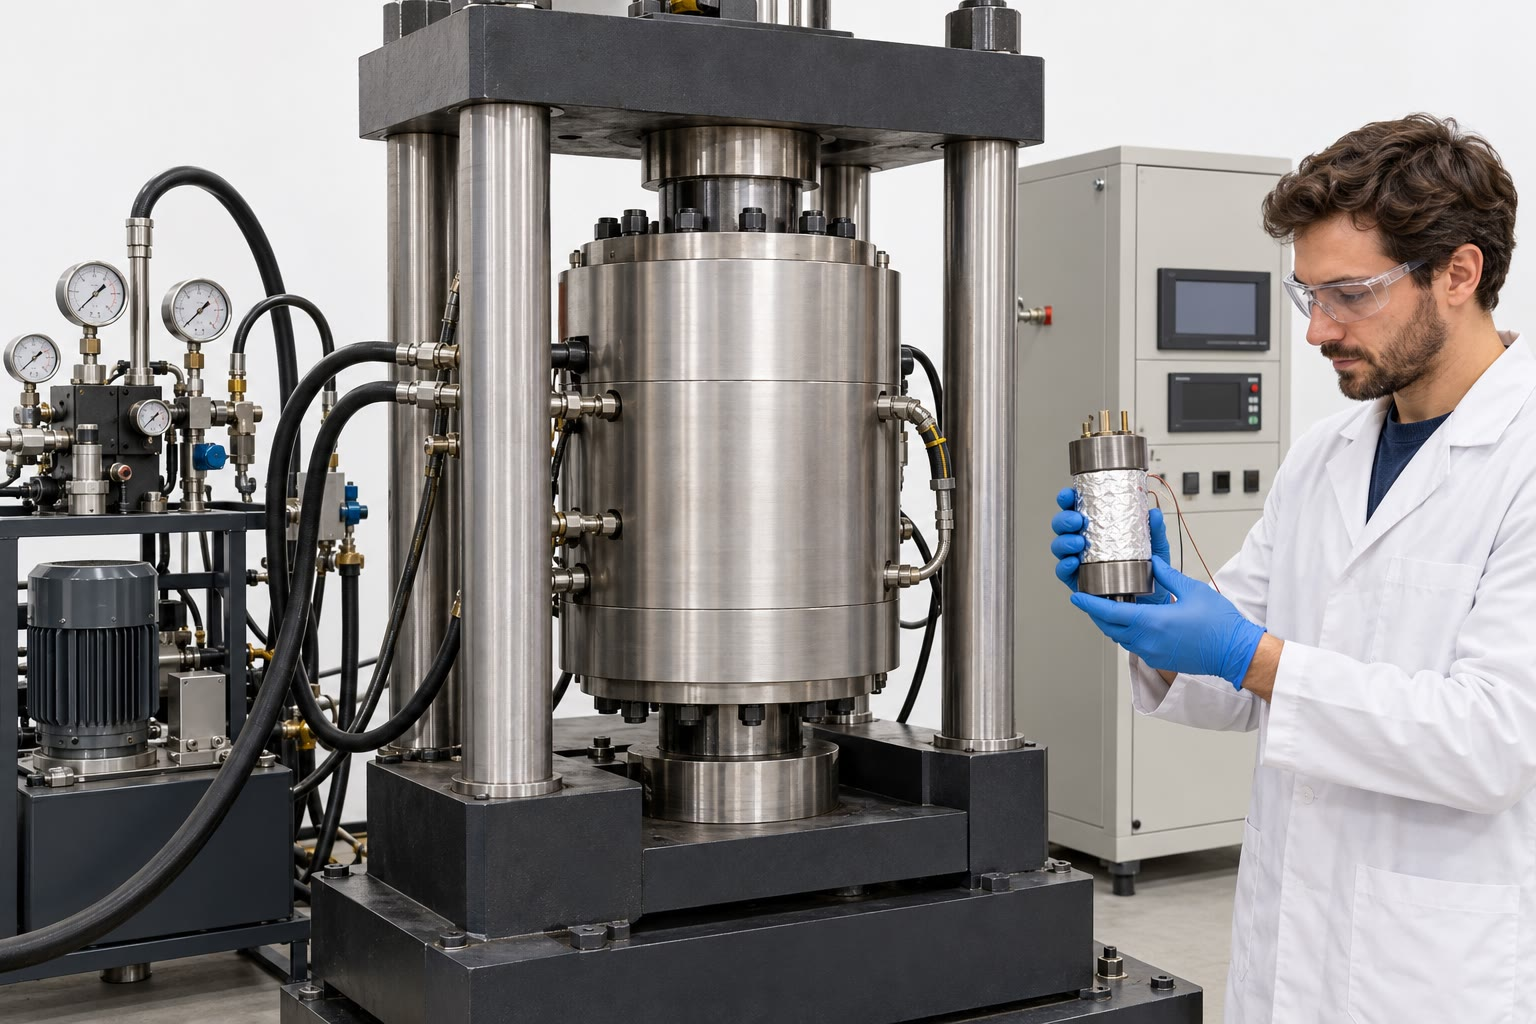
\includegraphics[width=\linewidth]{images/book5/ai/b3-deformation-press.jpg}

{\scriptsize खोलयुक्त नमूना संरचना वाला एक चट्टान-विरूपण प्रेस
(AI से बनाया गया चित्रण)।}

\smallskip
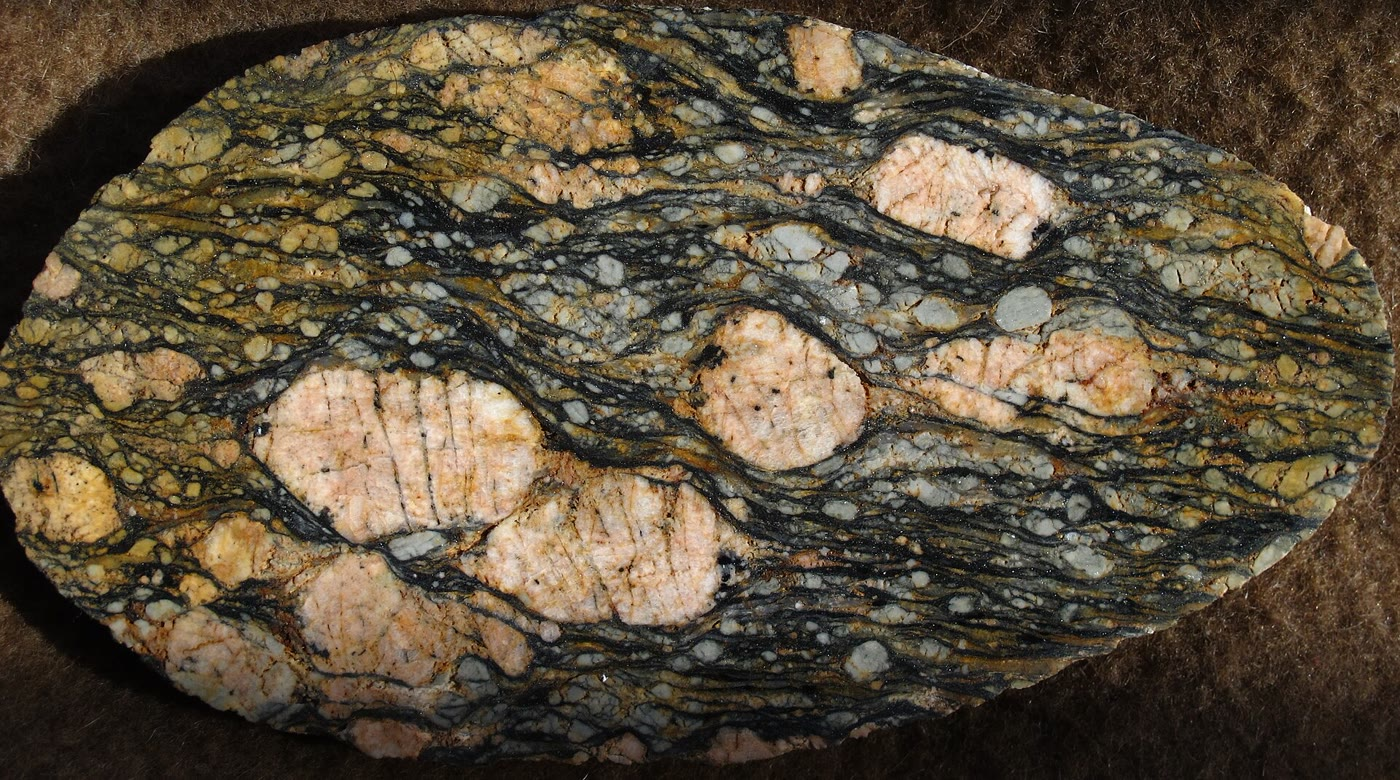
\includegraphics[width=\linewidth]{images/book5/b3-augen-mylonite.jpg}

{\scriptsize नॉर्वे का कटा हुआ ऑगन मायलोनाइट: बड़े फ़ेल्सपार पॉर्फ़िरोक्लास्ट
पुनःक्रिस्टलित क्वार्ट्ज़, फ़ेल्सपार और अभ्रक के बारीक आधार में। फ़ोटो
Mikenorton, CC BY-SA 4.0।}
\end{minipage}
\end{inthelab}
% ledger: mk00:diffusion, photo:b3-augen-mylonite

\section{अभ्यास}

\begin{exercise}[$\star$]\label{exo:b3:deformation-mechanisms:1}
\qty{1890}{\celsius} पर फ़ोर्स्टेराइट और \qty{0}{\celsius} पर बर्फ़ पिघलते हैं।
\qty{1300}{\celsius} पर फ़ोर्स्टेराइट का और \qty{-10}{\celsius} पर बर्फ़ का \omterm{def:b3:deformation-mechanisms:flow-law}{समजात तापमान} परिकलित कीजिए।
कौन अधिक आसानी से विसर्पित होता है?
\end{exercise}

\begin{exercise}[$\star$]\label{exo:b3:deformation-mechanisms:2}
\omterm{def:b3:deformation-mechanisms:shear-zone}{अपरूपण क्षेत्र} को समकोण पर काटने वाला एक डाइक क्षेत्र के भीतर \ang{70} से विक्षेपित होता है, और एक अन्य
\ang{80} से। कर्तन-विकृतियाँ परिकलित कीजिए। इस विधि से बड़ी
विकृतियों को मापना कठिन क्यों है?
\end{exercise}

\begin{exercise}[$\star$]\label{exo:b3:deformation-mechanisms:3}
क्वार्ट्ज़ दाबमापी के साथ, \qty{10}{\micro m} का
पुनःक्रिस्टलित कण-आकार किस प्रतिबल को इंगित करता है?
\end{exercise}

\begin{exercise}[$\star$]\label{exo:b3:deformation-mechanisms:4}
आर्द्र क्वार्ट्ज़ाइट के \omterm{def:b3:deformation-mechanisms:flow-law}{प्रवाह नियम} ($A = \num{1.1e-4}$, $n = 4$, $E =
\qty{223}{kJ.mol^{-1}}$, $R = \qty{8.314}{J.mol^{-1}.K^{-1}}$) की सहायता से,
\qty{20}{MPa} के अंतर्गत \qty{500}{\celsius} पर विकृति दर परिकलित कीजिए।
\end{exercise}

\begin{exercise}[$\star\star$]\label{exo:b3:deformation-mechanisms:5}
\qty{e-14}{s^{-1}} पर प्रवाहित होते आर्द्र क्वार्ट्ज़ाइट की प्रभावी श्यानता
\qty{400}{\celsius} (\qty{65.4}{MPa}) और
\qty{500}{\celsius} (\qty{18.0}{MPa}) पर परिकलित कीजिए, तथा इन्हें
\cref{ch:b3:mantle-convection} में दी गई प्रावार श्यानताओं से तुलना कीजिए।
\end{exercise}

\begin{exercise}[$\star\star$]\label{exo:b3:deformation-mechanisms:6}
समान तापमान पर दो प्रयोग \qty{100}{MPa} के अंतर्गत \qty{e-5}{s^{-1}} और
\qty{200}{MPa} के अंतर्गत \qty{1.6e-4}{s^{-1}} देते हैं। \omterm{def:b3:deformation-mechanisms:flow-law}{प्रतिबल घातांक} परिकलित कीजिए और
संभावित क्रियाविधि का नाम बताइए।
\end{exercise}

\begin{exercise}[$\star\star$]\label{exo:b3:deformation-mechanisms:7}
समान प्रतिबल पर एक नमूना \qty{1100}{K} पर, \qty{1000}{K} की तुलना में
दस गुना तेज़ विसर्पित होता है। सक्रियण ऊर्जा परिकलित कीजिए।
\end{exercise}

\begin{exercise}[$\star\star$]\label{exo:b3:deformation-mechanisms:8}
कण-आकार को दस से भाग देने पर \omterm{def:b3:deformation-mechanisms:creep}{विसरण विसर्पण} की विकृति दर किस गुणक से
बदलती है, नाबारो--हेरिंग और कोबल विसर्पण के लिए? कोबल विसर्पण
अधिक संवेदी क्यों है?
\end{exercise}

\begin{exercise}[$\star\star$]\label{exo:b3:deformation-mechanisms:9}
शुष्क ओलिवीन के लिए \qty{1100}{\celsius} और \qty{2}{GPa} पर दोनों \omterm{def:b3:deformation-mechanisms:flow-law}{प्रवाह नियम} देते हैं
$\dot\varepsilon_{\mathrm{dis}} = \num{6.54e-17}\,\sigma^{3.5}$ और
$\dot\varepsilon_{\mathrm{dif}} = \num{3.59e-6}\,\sigma d^{-3}$ (पाठ की
इकाइयों में)। $d = \qty{1}{mm}$ और $d =
\qty{100}{\micro m}$ के लिए सीमा-प्रतिबल, और सीमा की ढलान परिकलित कीजिए।
\end{exercise}

\begin{exercise}[$\star\star\star$]\label{exo:b3:deformation-mechanisms:10}
\cref{prop:b3:deformation-mechanisms:grain-size} की उपपत्ति के आधार पर,
जालक पथ $d^{-2}$ और सीमा पथ $d^{-3}$ क्यों देता है, यह समझाइए, और
यह दिखाइए कि कण-आकार $d^* \approx
(B_B/B_L)\,\delta D_B/D_L$ से नीचे सीमा विसरण प्रबल होता है।
\end{exercise}

\begin{exercise}[$\star\star\star$]\label{exo:b3:deformation-mechanisms:11}
$n = 3.5$ वाले \omterm{def:b3:deformation-mechanisms:flow-law}{प्रवाह नियम} के लिए प्रभावी श्यानता किस गुणक से घटती है,
जब विकृति दर को दस गुना किया जाता है? यह क्यों
विकृति के अपरूपण क्षेत्रों में स्थानीकरण को अनुकूल बनाता है?
\end{exercise}

\begin{exercise}[$\star\star\star$]\label{exo:b3:deformation-mechanisms:12}
अभ्यास 9 के शुष्क ओलिवीन में, \qty{10}{MPa} के अंतर्गत एक प्रावार \omterm{def:b3:deformation-mechanisms:shear-zone}{अपरूपण क्षेत्र}
\qty{3}{mm} से \qty{30}{\micro m} कणों में पुनःक्रिस्टलित होता है। कुल
विकृति दर पहले और बाद में, तथा \omterm{def:b3:deformation-mechanisms:shear-zone}{विकृति मृदुलन} का गुणक परिकलित कीजिए। कौन-सी
क्रियाविधि प्रत्येक स्थिति में विरूपण का वहन करती है?
\end{exercise}

\section{समस्या: वार्डन अपरूपण क्षेत्र}

\begin{problem}[{सप्ताहांत समस्या --- विकृति, प्रतिबल, विकृति दर और आयु
एक काल्पनिक अपरूपण क्षेत्र की}]
\label{pb:b3:deformation-mechanisms:1}
% values: calc/ch07.py; flow_laws.py; st03:piezometer, lopez:flow-laws
वार्डन पहाड़ियों के ग्रेनाइट के नीचे, श्रेणी के काल्पनिक क्षेत्र में, एक
बोरछिद्र और एक गहरी सड़क-कटान (दोनों काल्पनिक) से पता चलता है कि
यहाँ लगभग \qty{15}{km} गहराई और \qty{450}{\celsius} पर बना, \qty{400}{m} चौड़ा एक तन्य \omterm{def:b3:deformation-mechanisms:shear-zone}{अपरूपण क्षेत्र} है।
डोलेराइट का एक डाइक, जो दीवारों को समकोण पर काटता है, \omterm{def:b3:deformation-mechanisms:shear-zone}{अपरूपण क्षेत्र} के भीतर
उसकी सीमाओं से केवल \ang{6} का कोण बनाता है। इसका क्वार्ट्ज़ एक मायलोनाइट है,
जिसके पुनःक्रिस्टलित कणों का व्यास \qty{20}{\micro m} है (15 से
\qty{25}{\micro m} तक)। क्वार्ट्ज़ दाबमापी $D = 10^{3.56}\sigma^{-1.26}$ मान लीजिए,
आर्द्र क्वार्ट्ज़ाइट का \omterm{def:b3:deformation-mechanisms:flow-law}{प्रवाह नियम} ($A = \num{1.1e-4}$, $n = 4$, $E =
\qty{223}{kJ.mol^{-1}}$), $R = \qty{8.314}{J.mol^{-1}.K^{-1}}$, \qty{1}{yr} $=
\qty{3.156e7}{s}$, और सरल कर्तन में $\dot\gamma = 2\dot\varepsilon$।

\medskip\noindent\textbf{भाग I --- विकृति।}
\begin{enumerate}
  \item डाइक का विक्षेप $\psi$ और अपरूपण विकृति परिकलित कीजिए।
  \item एक दीवार का दूसरी के सापेक्ष विस्थापन परिकलित कीजिए।
  \item विकृति-दीर्घवृत्त के मुख्य स्ट्रेच और उसका अक्षीय
        अनुपात परिकलित कीजिए।
  \item क्षेत्र के साथ दीर्घ अक्ष का कोण परिकलित कीजिए।
        जैसे-जैसे $\gamma$ बढ़ता है, क्षेत्र का पर्णन क्या करता है?
  \item ऊपर से देखने पर, दक्षिणी दीवार से अनुसरण करने पर डाइक
        पूर्व-पश्चिम क्षेत्र में प्रवेश करते समय पूर्व की ओर मुड़ता है, फिर
        उत्तरी दीवार पर अपने उत्तरी मार्ग पर लौटता है। उत्तरी दीवार किस दिशा में
        खिसकी, और क्षेत्र दाएँ-पार्श्वीय है या बाएँ-पार्श्वीय?
  \item शुद्धगतिक सूचकों को पढ़ने के लिए पतली काट किस तल में बनानी चाहिए,
        और उसका S पर्णन किस प्रकार झुका होना चाहिए?
\end{enumerate}

\medskip\noindent\textbf{भाग II --- प्रतिबल।}
\begin{enumerate}[resume]
  \item \qty{20}{\micro m} कणों द्वारा संकेतित प्रतिबल परिकलित कीजिए।
  \item 15 और \qty{25}{\micro m} के लिए प्रतिबल परिकलित कीजिए।
  \item क्या प्रतिबल अंशांकन के परास के भीतर है?
  \item दाबमापी पर तापमान का कोई प्रभाव नहीं दिखा।
        यहाँ इसका क्या महत्व है?
  \item \qty{100}{MPa} के प्रतिबल से किस कण आकार का निर्माण हुआ होता?
\end{enumerate}

\medskip\noindent\textbf{भाग III --- विकृति दर।}
\begin{enumerate}[resume]
  \item \qty{450}{\celsius} पर $E/RT$ और आरेनियस गुणक परिकलित कीजिए।
  \item प्रश्न 7 के प्रतिबल के अंतर्गत क्वार्ट्ज़ की विकृति दर परिकलित कीजिए
        (\qty{62}{MPa} लीजिए)।
  \item अपरूपण विकृति दर परिकलित कीजिए।
  \item क्षेत्र की प्रभावी श्यानता परिकलित कीजिए और उसकी तुलना
        \cref{ch:b3:mantle-convection} के ऊपरी प्रावार से कीजिए।
  \item समान प्रतिबल पर, 400 और
        \qty{500}{\celsius} पर विकृति दर किन गुणकों से बदलेगी?
  \item यदि प्रतिबल सबसे बारीक कणों का
        \qty{78}{MPa} होता, तो किस गुणक से?
\end{enumerate}

\medskip\noindent\textbf{भाग IV --- समय।}
\begin{enumerate}[resume]
  \item प्रश्न 1 की अपरूपण विकृति संचित करने में लगा समय
        सेकंड में परिकलित कीजिए।
  \item उसे हज़ार वर्षों में बदलिए।
  \item क्षेत्र में माध्य विस्थापन दर परिकलित कीजिए, \unit{mm/yr} में।
  \item उसकी तुलना प्लेट-सीमाओं की उन दरों से कीजिए जो प्रति वर्ष दसियों मिलीमीटर होती हैं।
        % ledger: morvel:range
  \item यदि क्षेत्र \qty{20}{mm/yr} वहन करता, तो उसकी अपरूपण विकृति दर, प्रतिबल
        और पुनःक्रिस्टलित कण आकार क्या होते?
  \item कण आकार और दाबमापी के घातांक की अनिश्चितताएँ
        समय को कैसे प्रभावित करती हैं?
  \item वार्डन \omterm{def:b3:deformation-mechanisms:shear-zone}{अपरूपण क्षेत्र} को अपनी विकृति संचित करने में लगा समय,
        हज़ार वर्षों में दीजिए।
\end{enumerate}
\end{problem}
